\section{La librairie JPEG}
\subsection{Accès aux coefficients DCT}
Afin de réaliser le projet, notre professeur nous a fourni une librairie permettant la manipulation de fichiers JPEG. Ainsi, nous pouvons retrouver la structure suivante contenant différentes informations sur l'image en cours d'utilisation :
\begin{lstlisting}[language=C,style=customc]
typedef struct JPEGimg_s
{
	JBLOCKARRAY * dctCoeffs; // This is a 4-dimansion array. A coeff value is available in <structName>.dctCoeffs[comp][lin][col][pos]
	struct jpeg_decompress_struct cinfo; // Image informations such as number of components, size etc.
	jvirt_barray_ptr * virtCoeffs; // /!\ Do not modify this pointer of content /!\.
} JPEGimg; 
\end{lstlisting}
Après analyse de cette structure, nous savons que les coefficients DCT sont contenu dans le tableau à quatre dimensions \textit{dctCoeffs}. Ainsi, si nous souhaitons modifier un coefficient DCT, il suffit de réaliser l'opération suivante :
\begin{lstlisting}[language=C, style=customc]
for(i = 0; i < 8*8; i++){
    img->dctCoeffs[1][x][y][i]=a;
}
\end{lstlisting}
Où $x$ et $y$ sont les coordonnées du coefficient DCT dont nous voulons changer la valeur par $a$. La boucle $for$ nous permet d'affecter cette valeur à chaque pixel du bloc.\\
Si l'on souhaite remettre à zéro le bloc DCT du coefficient nous pouvons utiliser la fonction suivante :
\begin{lstlisting}[language=C, style=customc]
int rst_dct_block (JPEGimg *img, int block)
{
    int i,j,k;

    if (block > img->cinfo.num_components-1){
	char s[1];
	sprintf(s, "%d", block);
	print_err ("rst_dct_block()", s, ERR_RST_DCTB);
	return 1;
    }else{
	for (i = 0; i < img->cinfo.comp_info[block].height_in_blocks; i++){
	    for (j = 0; j < img->cinfo.comp_info[block].width_in_blocks; j++){
		for (k = 0; k < 64; ++k){
		    img->dctCoeffs[block][i][j][k]=0;
		}
	    }
	}
	return 0;
    }
}
\end{lstlisting}
Ainsi, nous pouvons obtenir les images suivantes en remettant le bloc DCT des trois coefficients de l'image de test suivante :
\begin{figure}[H]
    \centering
    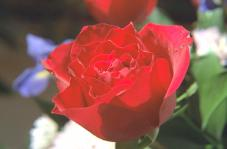
\includegraphics[width=.7\textwidth]{../SRC/testorig.jpg}
    \label{img:1}
    \caption{Image originale}
\end{figure}

\begin{figure}[H]
    \centering
    \begin{subfigure}[b]{0.3\textwidth}
        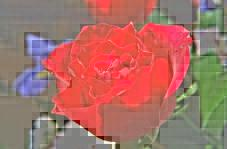
\includegraphics[width=\textwidth]{../SRC/test_b0.jpg}
        \caption{Coefficient DCT de la composante 1 à zéros ~($Y$)}
        \label{img:2}
    \end{subfigure}
    ~ %add desired spacing between images, e. g. ~, \quad, \qquad, \hfill etc. 
      %(or a blank line to force the subfigure onto a new line)
    \begin{subfigure}[b]{0.3\textwidth}
        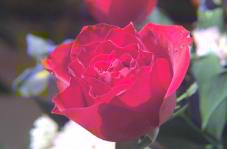
\includegraphics[width=\textwidth]{../SRC/test_b1.jpg}
        \caption{Coefficient DCT de la composante 2 à zéros ($Cb$)}
        \label{img:3}
    \end{subfigure}
    ~ %add desired spacing between images, e. g. ~, \quad, \qquad, \hfill etc. 
    %(or a blank line to force the subfigure onto a new line)
    \begin{subfigure}[b]{0.3\textwidth}
        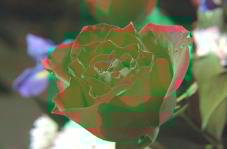
\includegraphics[width=\textwidth]{../SRC/test_b2.jpg}
        \caption{Coefficient DCT de la composante 3 à zéros ($Cr$)}
        \label{img:4}
    \end{subfigure}
    \caption{Résultats de la mise à zéro des coefficients DCT en fonction des composantes}\label{fig:lvl}
\end{figure}
Après avoir réalisé plusieurs tests sur plusieurs coefficients, nous avons pu remarquer que ceux qui influent le plus sur l'image sont ceux situés au début de la matrice du bloc (position $\left(0;0\right)$). Lorsque l'on altère ces composantes uniquement, on peut remarquer une perte considérable dans les couleurs de la composante choisie. On peut alors remarquer l'impact des différents coefficients DCT sur l'image lorsque ceux-ci sont remis à zéro :
\begin{figure}[H]
    \centering
    \begin{subfigure}[b]{0.3\textwidth}
        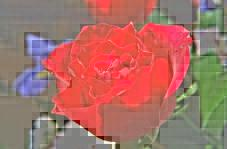
\includegraphics[width=\textwidth]{img/tot0.jpg}
        \caption{Premier coefficient DCT à zéro}
        \label{img:5}
    \end{subfigure}
    ~ %add desired spacing between images, e. g. ~, \quad, \qquad, \hfill etc. 
      %(or a blank line to force the subfigure onto a new line)
    \begin{subfigure}[b]{0.3\textwidth}
        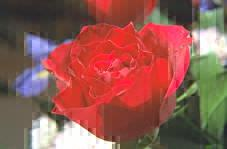
\includegraphics[width=\textwidth]{img/tot1.jpg}
        \caption{Second coefficient DCT à zéro}
        \label{img:6}
    \end{subfigure}
    ~ %add desired spacing between images, e. g. ~, \quad, \qquad, \hfill etc. 
    %(or a blank line to force the subfigure onto a new line)
    \begin{subfigure}[b]{0.3\textwidth}
        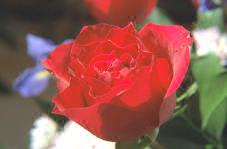
\includegraphics[width=\textwidth]{img/tot10.jpg}
        \caption{Dixième coefficient DCT à zéro}
        \label{img:7}
    \end{subfigure}
    \caption{Influence des différents blocs DCT}\label{fig:DCT}
\end{figure}
